Probabilistic Seismic Hazard is nowadays a well established methodology, largely 
founded on the works of \citeauthor{cornell1968} and \citeauthor{esteva1968}, 
both published at the end of the 1960's. 
%
The development of PSHA within the latest four decades did not change much the 
original concept but made calculations more rigorous and accurate, especially 
with respect to the treatment of uncertainties. 

The evolution of PSHA methodologies proceeded in parallel with the development 
of instrumental seismology and hardware computing power. Computer codes such as
EQRISK \citep{mcguire1976} and different SEISRISK versions 
\citep{bender1982,bender1987} traced the advancement of PSHA calculation within
the last part of the 20th century.

At the present time, the most computationally intensive PSHA models available 
are the ones developed for site-specific PSHA analyses, such as the ones 
performed for special installations, and the regional PSHA input models. 
In the first case most of the computation demand comes from the complexity 
of the input whilst in the second case is the number of sites considered that 
makes calculations particularly heavy.  
%
% ------------------------------------------------------------------------------
\section{OpenQuake-hazard: main concepts}
OpenQuake-hazard leverages from OpenSHA (http://www.opensha.org) - an 
open-source, Java-based platform for conducting Seismic Hazard Analysis - and 
it is developed in collaboratio30n with the OpenSHA team. 

Schematically, the procedure that OpenQuake follows to compute the hazard is 
the following:
%
\begin{enumerate}
%
\item \emph{Read the PSHA input model - i.e. the union of the Seismic Sources 
System and the Ground Motion Model System - and calculation 
settings.}
	\index{Seismic Sources!System} %%%%%%
	\index{PSHA!Input model} %%%%%%
	\index{Ground Motion!Model!System} %%%%%%
	%
	The \emph{Seismic Sources System} is an object that contains the 
	information necessary to create one or several Seismic Sources Model, 
	eventually by taking into account the epistemic uncertainties. 
	%
	In particular, the Seismic Sources System contains:
	\begin{itemize}
	\item One or several \emph{Initial Seismic Sources Models};
	\index{Logic Tree!Seismic sources} %%%%%%
	\item One logic tree - the Seismic Sources Logic Tree - describing 
	epistemic uncertainties connected with the objects and parameters 
	characterizing the Initial Seismic Sources Models.
	\end{itemize}
	%
	The Ground Motion Model System is an object that contains the information 
	necessary to create (or use) one or several Ground Motion models, eventually 
	by taking into account the epistemic uncertainties. 
	\begin{itemize}
	\item One or several Ground Motion Models;
	\index{Logic Tree!Ground Motion Model} %%%%%%
	\item One logic tree - the Ground Motion Model Logic Tree - 
	describing epistemic uncertainties connected with the objects and 
	parameters characterizing the selected Ground Motion Models.	
	\end{itemize}

%
\item \emph{Process the logic tree structures to account for epistemic 
uncertainties connected with the seismic sources and the ground motion 
prediction equations and, create Seismic Sources Models and Ground Motion 
Prediction Equations Models}.
	\index{Seismic Sources!Model} %%%%%%
	\index{Ground Motion! Prediction Equations!Model} %%%%%%
	%
	A Seismic Sources Model contains the information necessary to create an 
	Earthquake Rupture Forecast (i.e. the probabilistic seismicity occurrence
	model) without considering any epistemic uncertainty.
	%
	A Ground Motion Prediction Equations Model includes the information 
	necessary to compute hazard using a Seismic Sources Model. 
\item Compute the hazard considering as many Seismic Sources Models and 
Ground Motion Prediction Equations Models as need to adequately characterize 
uncertainties.
\item Post-process the results obtained for distinct calculations.
\end{enumerate}
%
% ------------------------------------------------------------------------------
\section{Calculation workflows}
% Three types of analysis
The OpenQuake-Hazard module offers the capability to perform seismic hazard 
analysis (SHA) following various approaches. Currently three main types of 
analysis are supported:
\begin{itemize}
\item \textbf{Classical probabilistic SHA}, allowing calculation of hazard 
curves and hazard maps following classical integration procedure 
(\cite{cornell1968}) as formulated by \cite{field2003}.
\item \textbf{Event-Based probabilistic SHA}, allowing calculation of ground 
motion fields from stochastic event sets.
\item \textbf{Deterministic SHA}, allowing calculation of ground motion fields 
from single earthquake rupture scenario.
\end{itemize}
Each type of analysis involves a number of calculators, each responsible for 
a specific task. Figures \ref{classical_psha_workflow}, 
\ref{event_based_workflow}, and \ref{deterministic_workflow} 
schematically depict the different calculation workflows. \\
% Classical and Event based : Input Data Definition
For both the the classical and event-based probabilistic SHA 
(hereinafter PSHA), the input data consist of a seismic hazard model structured 
in terms of a source model logic tree (representing the seismicity model and 
the associated epistemic uncertainties) and a ground motion model logic tree 
(representing the ground motion model utilized for ground shaking estimation 
and the associated epistemic uncertainties).\\
% Seismicity Model
A seismicity model consists of a collection of seismogenic sources. 
A seismogenic source can be one of four typologies: area, point, simple fault, 
and complex fault. An area source represents a geographic region where 
seismicity is assumed to be uniform. A point source models a single 
geographical location of concentrated seismicity. A collection of point sources 
or area sources can be used to model distributed seismicity. 
Seismicity occurring on recognized fault structures can be modeled in terms of 
simple fault (for a geometrically regular-shaped fault), or as complex fault 
(allowing modeling of a more geometrically irregular fault structure). 
Each seismogenic source is also associated to a tectonic region type.\\
% Ground Motion Model
A ground motion model is defined as a collection of ground motion prediction 
equations (GMPEs), each one associated to a specific tectonic region type (for 
instance: shallow active crust, stable continental region, subduction interface,
subduction intraslab, volcanic). The definition of a tectonic region type allows
linking a seismogenic source with the appropriate GMPE.\\
% Epistemic uncertainties
Epistemic uncertainties in the source model...
% Logic Tree processor
Such data is then passed to the Logic Tree Processor that is responsible for 
'harvesting' the information contained in the logic tree structure, that is
to sample the epistemic uncertainties so that the distribution of the final 
hazard results reflect the uncertainties in the seismicity and ground motion
models. Once a source model is selected from the logic tree, it is subsequently 
used as input for the Earthquake Rupture Forecast (ERF) calculator which 
computes the probability of occurrence, over a specified time span, for each 
earthquake rupture contained in the source model. Such inventory of all the 
ruptures defined in the source model, with their probabilities of occurrence, 
is referred to as ERF.\\
When performing a classical PSHA, the ERF is provided as input (together with 
a ground motion model) to the the Hazard Curve Calculator which compute 
probabilities of exceeding a set of ground motion values (that is an hazard
curve) by summing the contribution from all the earthquake ruptures contained
in the ERF. For the event-based PSHA instead, the Stochastic Event Set 
Calculator generates stochastic event sets by sampling each rupture contained 
in the ERF according to its probability of occurrence. For each event in the 
event set, the Ground Motion Field Calculator computes a realization of the 
ground shaking taking into account the aleatory uncertainties in the ground 
motion model.\\
% Deterministic
For deterministic SHA (DSHA), the input data consist of a single earthquake 
rupture model and a single ground motion model. Using the Ground Motion Field 
Calculator, multiple realizations of ground shaking can be computed, each 
realization sampling the aleatory uncertainties in the ground motion model.\\
% Modular structure
Each type of analysis has a modular structure, thus providing the capability 
of investigating all possible intermediate results. Moreover, each calculator 
can be expanded independently so that more calculation options/methodologies 
can be easily introduced, without affecting the overall calculation workflow.\\
% More details in the next chapters
Next chapters discuss in more details the data model and the calculators. 
Chapter \ref{chap:idd} describe the input data definition, that is the 
different options for modeling seismogenic sources and how to include 
epistemic uncertainties in both seismicity and ground motion models in 
the form of a logic tree. The inclusion of epistemic uncertainties in 
the hazard calculations is described in Chapter \ref{chap:ltp}. The 
definition and modeling of earthquake ruptures for the different seismogenic 
source typologies is the topic of Chapter \ref{chap:erfc}. Chapter 
\ref{chap:hcc} describes the theoretical framework behind the hazard 
curve calculator. The main calculators for the event-based PSHA are 
described in Chapters \ref{chap:sesc} and \ref{chap:gmfc} (Stochastic 
Event Set Calculator, and Ground Motion Field Calculator respectively). 
Examples of classical PSHA, event-based PSHA, and DSHA are reported in 
Chapters \ref{chap:cpsha}, \ref{chap:ebpsah}, and \ref{chap:dsha}.
\begin{figure}[htbp]
\begin{center}
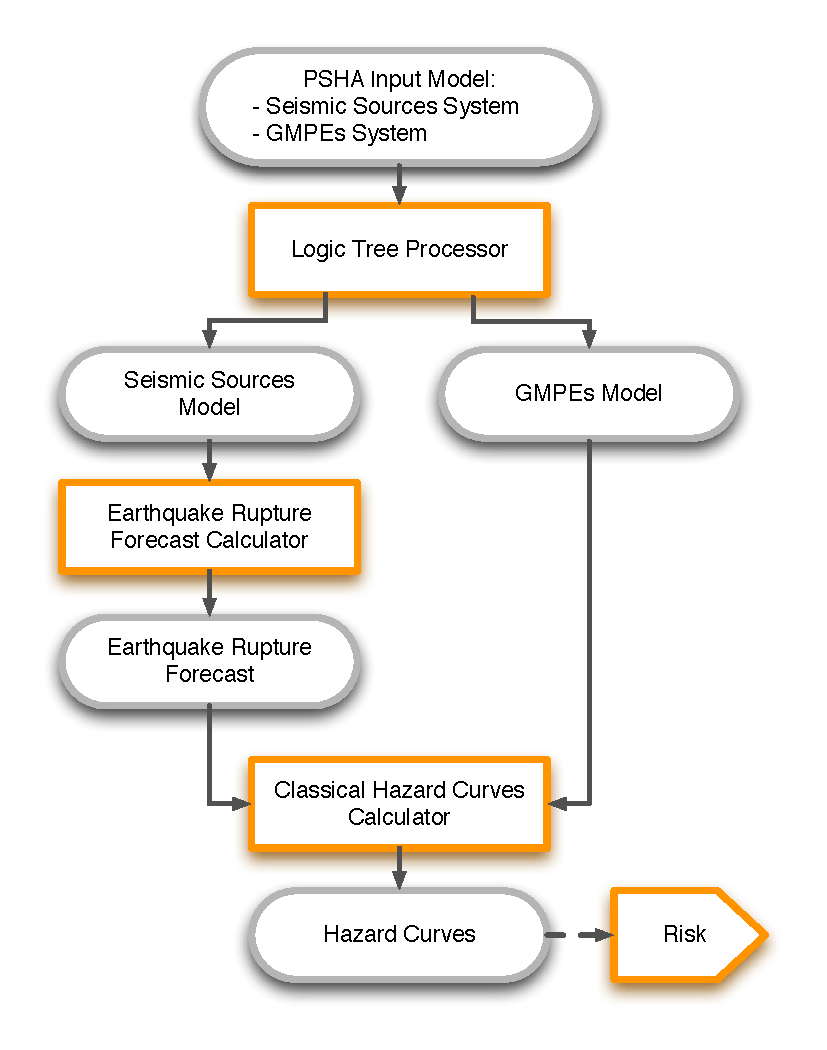
\includegraphics[width=10cm]{./Figures/Part_Hazard/classical_psha_workflow.eps}
\caption{Workflow for classical PSHA. Given a seismic hazard model 
(expressed as source and ground motion model logic trees), the Logic Tree 
Processor is responsible for selecting a particular source and ground motion 
models. The source model is then provided to the Earthquake Rupture Forecast 
calculator, which computes the ERF (the list of all earthquake ruptures in the 
source model with their probabilities of occurrence). Together with the selected 
GMPE hazard curves are calculated.}
\label{classical_psha_workflow}
\end{center}
\end{figure}
% 
\begin{figure}[htbp]
\begin{center}
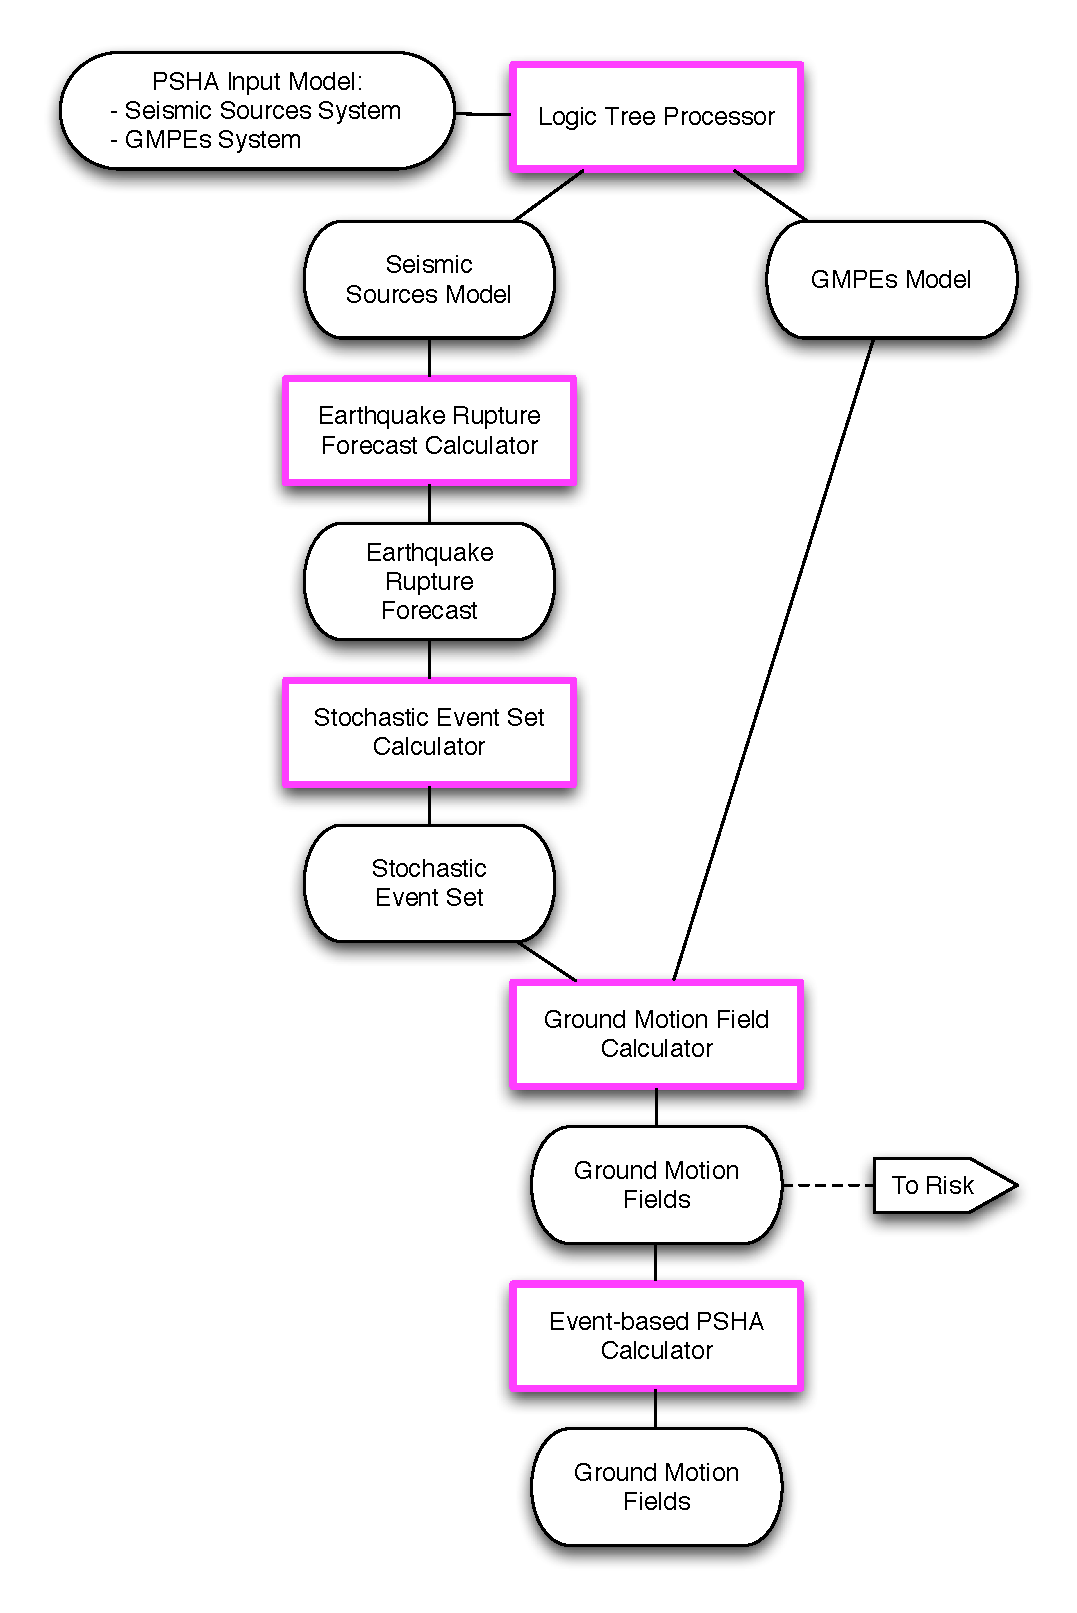
\includegraphics[width=7cm]{./Figures/Part_Hazard/event_based_workflow.eps}
\caption{Workflow for event-based PSHA. Similarly to the classical PSHA workflow 
(Figure \ref{classical_psha_workflow}), an ERF is computed, which is then used 
to generate a stochastic event set (representative of the seismic activity of 
a region in a given time span). Each event is then utilized to calculate a 
ground motion field over a region of interest.}
\label{event_based_workflow}
\end{center}
\end{figure}
%
\begin{figure}[htbp]
\begin{center}
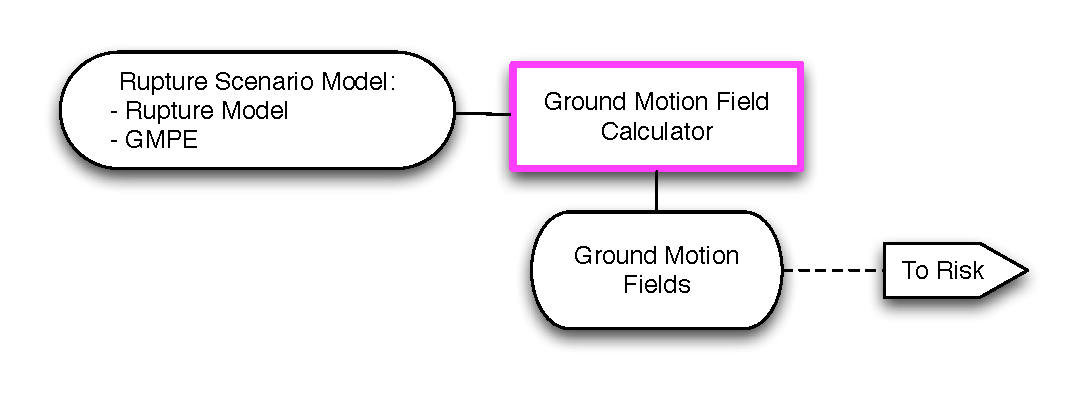
\includegraphics[width=7cm]{./Figures/Part_Hazard/deterministic_workflow.eps}
\caption{Workflow for deterministic SHA. Given a rupture scenario model, 
consisting of an earthquake rupture model, plus a GMPE, the ground motion 
field calculator can compute multiple ground motion field realizations (by 
taking into account GMPE aleatory uncertainties).}
\label{deterministic_workflow}
\end{center}
\end{figure}
%